\section{Background and Threat Model}%
\label{sec:background_and_threat_model}

% 这个章节也是由初稿中的Paranoma中分离出来,但是原来的全景图更换为威胁模型图,要重新写这部分内容
% This section presents some necessary background knowledge to facilitate readers to understand HyperPS and threat model better.

% depicted in Figure \ref{pic:panorama}.

\subsection{Background}%
\label{sub:background}

\subsubsection{QEMU-KVM}%
\label{ssub:qemu_kvm}
QEMU is a generic and open-source machine emulator and virtualizer. QEMU can use other hypervisors, like XEN or KVM, to use CPU extensions for virtualization. When used as a virtualizer, QEMU achieves near native performances by executing the guest code directly on the host CPU.
Kernel-based Virtual Machine (KVM) is an open-source virtualization technology that converts Linux into a type-1 (bare-metal) hypervisor. KVM is a part of the Linux kernel that shares all the Linux kernel's operating system-level components -such as the memory manager, process scheduler, security manager, and more to run VMs. Every VM is implemented as a regular Linux process, scheduled by the standard Linux scheduler, with dedicated virtual hardware like a network card, memory, and disks. KVM mainly consists of a loadable kernel module, kvm.ko, that provides the core virtualization infrastructure and a processor specific module, kvm-intel.ko or kvm-amd.ko.
In a virtualization environment, KVM does not work on its own. It is only an API provided by the kernel for userspace. End users typically use KVM through QEMU, where it is present as an acceleration method.
For the QEMU-KVM architecture, KVM interacts with QEMU (QEMU runs at the user space) in two ways: through device file \verb|/dev/kvm| and through memory mapped pages.
% KVM interacts with user space - in most case QEMU - in two ways: through device file \verb|/dev/kvm| and through memory mapped pages.
Memory mapped pages are used for bulk transfer of data between QEMU and KVM. \verb|/dev/kvm| is the main API exposed by KVM. It supports a set of \verb|ioctl|s which allow QEMU to manage VMs and interact with them.
% 怎么引出Hostos的问题
% Since KVM is a part of the linux kernel, the Linux and the QEMU
% leverages the linux kernel's system-level



\subsubsection{VMCS}%
\label{ssub:vmcs}
Virtual-machine Control Structure is a data structure used in Virtual Machine eXtensions (VMX). It controls VMX non-root operations (guest virtual machine execution operations) and VMX transitions. Access to the VMCS is managed through the VMCS pointer (one per logical processor). The VMCS pointer is read and written using the instructions \verb|VMPTRST| and \verb|VMPTRLD|. In general, the hypervisor configures a VMCS using \verb|VMREAD|, \verb|VMWRITE|, and \verb|VMCLEAR| instructions. A hypervisor could use a different VMCS for each virtual machine that it supports. For a virtual machine with multiple logical processors, the hypervisor could use a different for each logical processor. A logical processor may also maintain a number of VMCSs that are active, however, at any given time, at most one of the active VMCSs is the \textbf{current} VMCS. VMX instructions operate only on the \textbf{current} VMCS. 

%这段写的不好,没有写出危害的具体内容,应该突出VMCS就是唯一的接口,VM的所有的行为都是在VMCS的instruct下的
A compromised Hostos/hypervisor can force the guest virtual machine exit by tampering VM-Execution Control fields and VM-exit control fields in VMCS and tamper the guest virtual machine by writing Guest-State Area fields. 

% 一个被危害的hypervisor可以强迫虚拟机退出,并通过篡改其vmcs中的field等信息实现对guest VM 的危害。

% \subsection{Second Level Address Translation}%
% \label{sub:second_level_address_translation}
% Second Level Address Translation (SLAT) is a hardware-assisted virtualization technology which makes it possible to quick manage the physical memory without lots of VM exits. Extended Page Table (EPT) is the intel's implementation of SLAT, while ARM names its implementation as Stage-2 Page-tables.


\subsubsection{EPT}%
\label{ssub:ept}
Intel implements its Second Level Address Translation (SLAT) as Extended Page Table (EPT). 
EPT allows each virtual machine to manage its page table (not the EPT), without giving access to the underlying host machine's MMU Hardware. Thus, EPT reduces the need for hypervisor to keep syncing the shadow pages eliminating the overhead.
If EPT is enabled, guest-physical addresses are translated by traversing a set of EPT Paging-structures to produce physical addresses that are used to access memory.
In addition to translating a guest-physical address to a physical address, EPT specifies the privileges that software is allowed when accessing the address. Attempts at disallowed accesses are called EPT violations and cause VM exits.

A compromised Hostos/hypervisor could tamper EPT Paging-structures so that the virtual machine will execute arbitrary malicious code without knowing it. 
Moreover, a compromised Hostos/Hypervisor could access any data in the guest virtual machine with the help of virtual machine introspection.

\iffalse
\subsubsection{EPT Address Translation Mechanism}%
\label{ssub:ept_address_translation_mechanism}
When a logical CPU executes the guest code in non-root mode, the CPU loads the guest CR3 of the client process. Since the guest CR3 is a Guest Physical Address (GPA), the CPU needs to query the EPT page table to implement the guest CR3 GPA->HPA (Host Physical Adddress) conversion. 
the address used is the guest virtual address. the CPU in 
\fi



\subsubsection{EPTP Management}%
\label{ssub:eptp_management}
% 目前,对EPTP的管理有两种,
The extended-page-table pointer (EPTP) contains the address of the base EPT table, as well as other EPT configuration information. 
The value of EPTP is stored in the VM-Execution Control Fields of VMCS. 
The hypervisor can manage and configure EPTP value in VMX root operation, while Intel also provides \verb|VMFUNC| to allow software in VMX non-root operation to load a new value for the EPTP without VM-Exit.
% \verb|VMFUNC| is a new instruction introduced by intel. This intruction allows software in VMX non-root operation to invoke a VM function, which is processor functionality enabled and configured by the hypervisor in VMX root operation.
EPTP switching is VM function 0. EPTP switching allows software (in both kernel and user mode) in guest VM to directly load a new EPTP, thereby establishing a different EPT Paging-structure hierarchy. 
The value of EPTP can only be selected from a list of pre-configured values in advance by the hypervisor. 

% EPTP switching is one of these VM functions, which allows software (in both kernel and user mode) in guest VM to directly load a new EPTP, thereby establishing a different EPT Paging-structure hierarchy.




%\subsection{Attacks and Threat Model} \label{sub:thretmodel}
\subsection{Attack Surface}\label{sub:attacksurface}
\iffalse
在这一章节中,我们首先给出攻击者的攻击路径,这个攻击路径并不需要单独画图,因为上面的图中已经阐释清楚了,攻击者有哪些方式可以危害虚拟机,只需要在图中更加明确的标识出来就可以了。然后再给出本文的威胁模型。

首先一句话尽可能简洁的描述出攻击者的攻击目的,

在这一章节中,我们首先描述在云环境中,攻击者如何攻击利用Hostos的漏洞实现对客户虚拟机的攻击。
其次,我们给出敌手的能力。
\fi

In this section, we first present how attackers tamper virtual machines through exploiting vulnerabilities in Hostos/Hypervisor. Then, we present several typical attack models/examples targeting at VMCS and EPT. At last, we explain some additional attacks (not attacks relative to virtualization components)
% We present attack surface of hypervisor and

\begin{figure}[htpb]
    \centering
    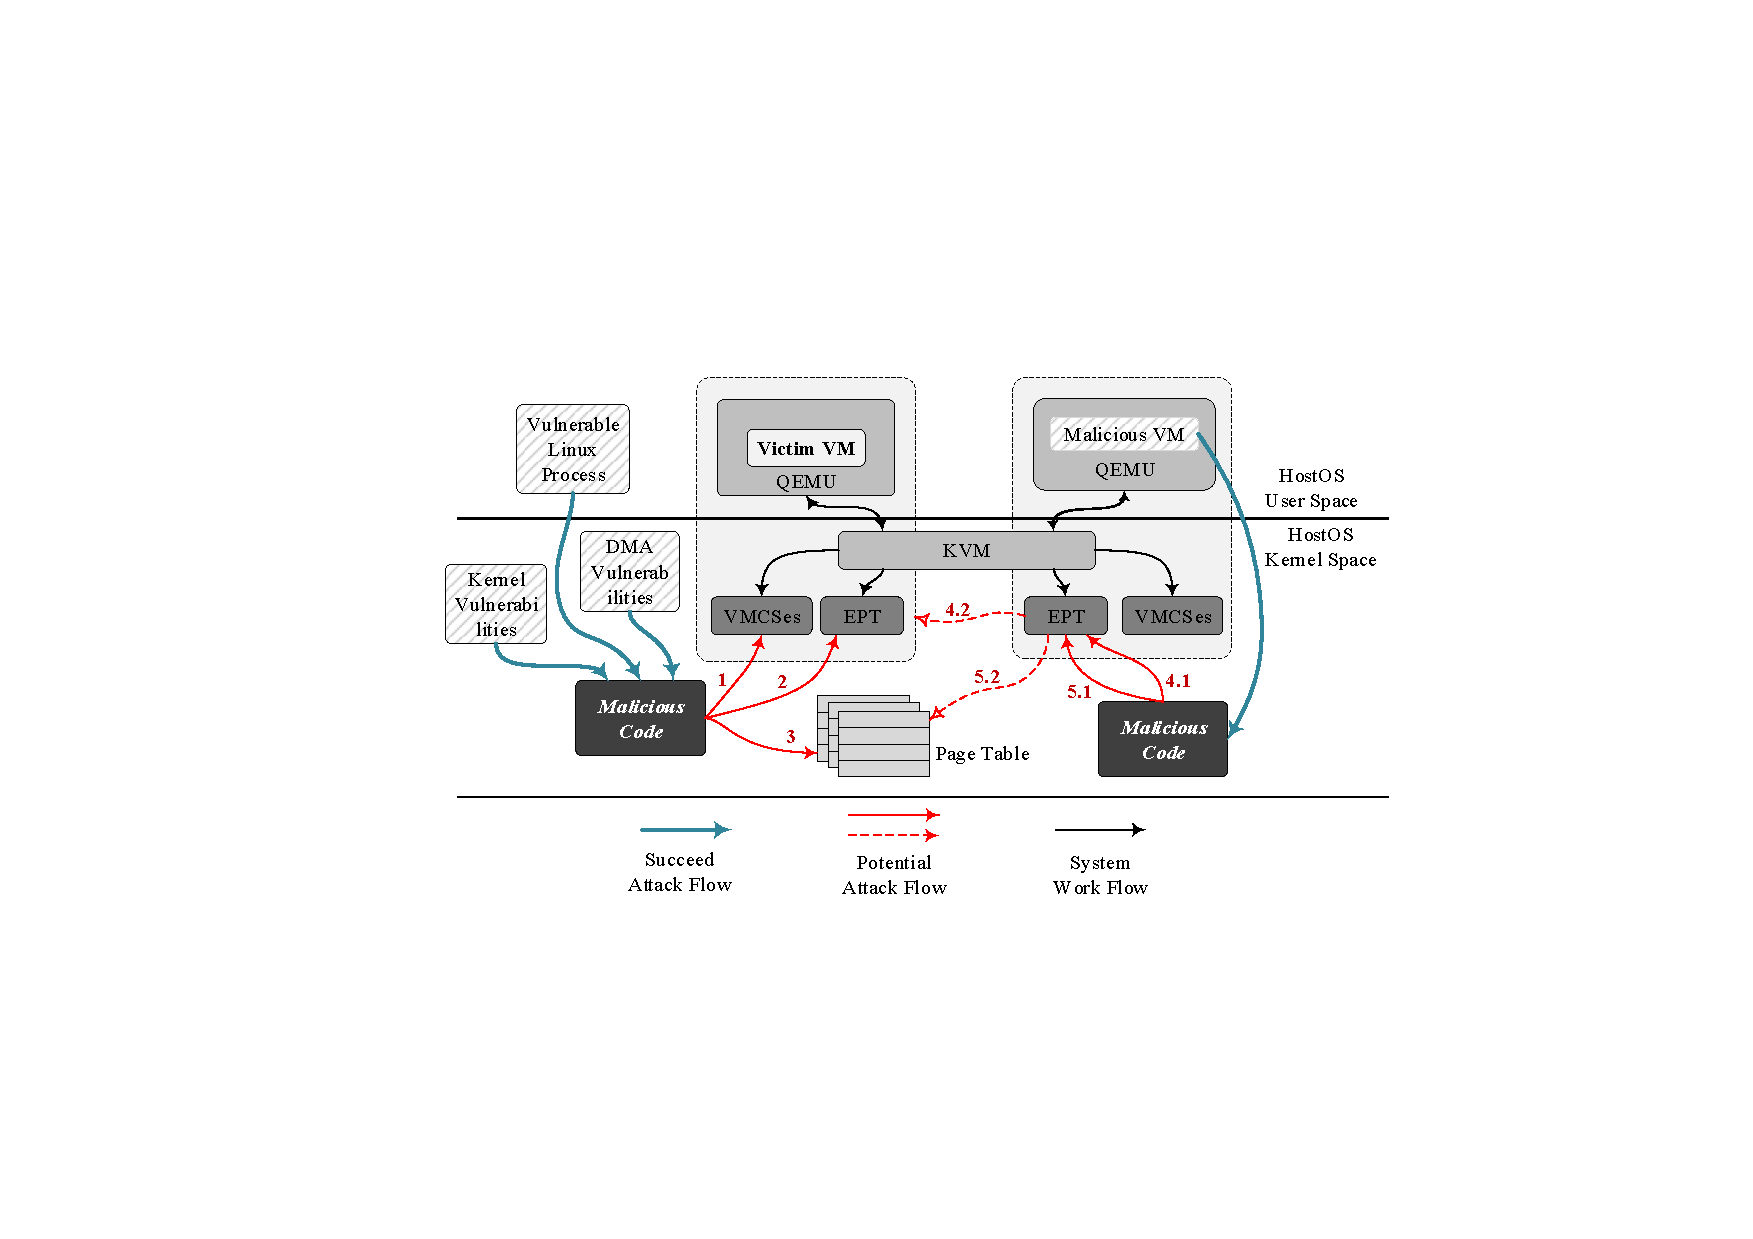
\includegraphics[width=1\linewidth]{IMG/threat.pdf}
    \caption{The Attack Paths in the QEMU-KVM Cloud Environment}%
    \label{fig:threat}
\end{figure}

% depicted in Figure \ref{pic:panorama}.
%将图中的具体的攻击名称 1 2 3 4 等添加进去。
%At last, we illustrate the adversary's abilities. 

\subsubsection{How attacker subvert VM}

\iffalse
%##########################################
% 老版本的内容,感觉更好,但是跟图不相符
%##########################################
As illustrated in Section \ref{sub:background}, Hypervisor manages VM's physical memory through EPT, and it configures and manages EPTs through the EPTP field in VMCS. Therefore, these two data structures: VMCS (especially the EPTP field) and EPT, become the key target for adversary to tamper VMs. 
% Hypervisor controls the execution of VMs through VMCSs, manages VMs' physical memory through EPT, and configures and manages EPTs through EPTP.
% As such, these two data structures become the key target for adversary to tamper VMs.
As depicted in Figure \ref{fig:threat}, 
An adversary can exploit vulnerabilities to ``jail-break'' into the Hostos/Hypervisor, while he can also subvert Hostos/Hypervisor by exploiting vulnerabilities in the Hostos (both the kernel and the user process).
In this paper, we hypothesize the Hostos/Hypervisor has already been compromised, we attempt to protect VMs under the compromised Hostos/Hypervisor. 
After compromising the Hostos/Hypervisor, the attacker will inject malicious code to subvert VMs by tampering EPTP field in VMCSes and EPTs.
In details, we assume that the attacker can tamper VMCSs and EPTs with one of the following methods. First, the attacker can tamper any field in these two data structures with \verb|VMX| instructions, if the attacker has gained the root processor privilege. 
Second, the attacker can tamper these two data structures through direct memory write operations. The attacker can write these two data structures either through Direct Memory Access (DMA) or through regular memory access, if the attacker acquired these two data structures' memory locations before.  
\fi

As illustrated in Section \ref{sub:background}, Hypervisor manages VM's physical memory through EPT, and it configures and manages EPTs through the EPTP field in VMCS. Therefore, these two data structures: VMCS (especially the EPTP field) and EPT, become the key target for an adversary to tamper VMs. 
In this paper, we emphasize that the attacker does not settle for the denial of service attack, but attempts to inject malicious code into the victim VM. 
Therefore, the memory, both it is access permissions and mapping relationships, is the most important target. 

As depicted in Figure \ref{fig:threat}, 
An adversary can exploit vulnerabilities to ``jail-break'' into the Hostos/Hypervisor, while he can also subvert Hostos/Hypervisor by exploiting vulnerabilities in the Hostos (both the kernel and the user process).
In this paper, we hypothesize the Hostos/Hypervisor has already been compromised, we attempt to protect VMs under the compromised Hostos/Hypervisor. 
After compromising the Hostos/Hypervisor, the attacker will inject malicious code to subvert VMs by tampering EPTP field in VMCSes and EPTs.
However, we do not restrict how attackers can compromise VMCSes or EPT. 
For example, an attacker can tamper any fields in VMCSes or EPT with \verb|VMX| instructions, if he has gained the root processor privilege. An attacker can also tamper these two data structures through memory write operations. We assume that the attacker can write these two data structures either through Direct Memory Access (DMA) or through regular memory access. 

% Figure \ref{pic:threat} shows how an attacker subverts a VM after the Hostos/Hypervisor has been exploited before.
As mentioned above, we emphasize memory security, so that we have detailed the various attack paths of attackers against EPT in Figure \ref{fig:threat}.
An attacker can tamper with the EPTP field in VMCS directly, thereby establishing a dedicated and malicious EPT Paging-structure hierarchy, which is the Attack Path 1 in Figure \ref{fig:threat}. 
The attacker can also tamper with EPT Paging-structures directly (Attack Path 2).
However, in some scenarios, the attacker does not have the ability to subvert the victim VM's VMCSes or EPT directly. 
In some cases, the attacker can only tamper with page tables, which is Path 3 in Figure \ref{fig:threat}. However, the VM's memory in the QEMU-KVM environment is not only managed by the EPT, but also managed by the Hostos's page tables (QEMU process's page tables). An attacker could subvert the victim VM by tampering with the corresponding QEMU process's page table entries. The situation would be extremely severe when the VM (QEMU process) requests a new memory area or delivers a page fault interruption. In this situation, Hostos page tables are involved because of page fault, EPT is involved because of establishing new EPT Paging-structure. 
In other cases,  
an attacker may only be able to modify the EPT Paging-structures of a malicious VM (Attack Path 4 and Attack Path 5 in Figure \ref{fig:threat}). 
The attacker could break the memory isolation between VM's by exploiting memory or page table vulnerabilities. For example, VMs with same guestos kernel may share the same kernel code memory frames. An attacker may subvert the victim VM by exploiting Copy-On-Write (COW) vulnerabilities in Hostos. 

\iffalse
share the same guestOS kernel code section in same physical memory frames
in some cases, A malicious VM may access to the 
map the the victim VM's memory into 
With memory vulnerabilities, 
The attacker could subvert the victim VM by 
the malicious VM's EPT 
map the victim VM's memory 
% describe in detail the
% memory-related
the memory 
For example, as shown Step 1 in Figure \ref{fig:threat}, an attacker can tamper with the EPTP field in VMCS directly, thereby establishing a dedicated and malicious EPT Paging-structure hierarchy.
The attacker can also tamper with EPT directly (Step 2).
, if the attacker acquired these two data structures' memory locations before.  
In details, we assume that the attacker has gained the root processor privilege, so that he can tamper any field in VMCSes or EPT with \verb|VMX| instructions. We also assume that 
In details, we assume that the attacker can tamper VMCSs and EPTs with one of the following methods. We does not limit the adversary 
First, the attacker can tamper any field in these two data structures with \verb|VMX| instructions, if the attacker has gained the root processor privilege. 
For example, as shown Step 1 in Figure \ref{fig:threat}, an attacker can tamper with the EPTP field in VMCS directly, thereby establishing a dedicated and malicious EPT Paging-structure hierarchy.
The attacker can also tamper with EPT directly (Step 2).
Second, the attacker can tamper these two data structures through direct memory write operations. The attacker can write these two data structures either through Direct Memory Access (DMA) or through regular memory access, if the attacker acquired these two data structures' memory locations before.  
For example, as shown Step 1 in Figure \ref{fig:threat}, an attacker can tamper with the EPTP field in VMCS directly, thereby establishing a dedicated and malicious EPT Paging-structure hierarchy.
The attacker can also tamper with EPT directly (Step 2).
Second, the attacker can tamper these two data structures through direct memory write operations. The attacker can write these two data structures either through Direct Memory Access (DMA) or through regular memory access, if the attacker acquired these two data structures' memory locations before.  
%direct write to fields in these two data structures or 
%在这里要修改图,图中要添加内核的其他部分的功能,去掉内部管理者,保留虚拟机逃逸部分,同时对这部分的内容做虚线处理。

%这里,我们给出几个攻击模型,举例说明攻击者是如何危害上面的虚拟机的。
\fi

\subsubsection{Attack Examples}
\label{ssub:attack_examples}
We present several attacks to illustrate how an attack subvert VMs by through tampering VMCS and EPT.

\textbf{VMCS Subversion}:
Attackers can tamper fields of VMCS in VM Exit stage. For example, modifying the value of \verb|HOST_RIP| register and writing a malicious program address to this register will cause a control flow hijacking attack. Modifying the value of privilege register, CR0, will close the DEP mechanism, and modifying the value of CR4 register will close the SMEP mechanism.


\textbf{EPT Subversion}: 
Malicious modification of EPT will break the isolation between virtual machines. A vicious VM can break the isolation between VMs by tampering with EPT entries, and access the memory of the victim VM at his vicious will. For example, the attacker can conduct remapping attack and double mapping attack to inspect a victim VM. 

For the double mapping attack, the attacker first controls and compromises a VM, then obtains the privilege of the hypervisor through the virtual machine escape attack, and maliciously accesses the VMCS structure to obtain the value of EPTP. The attack process is as shown in Figure \ref{pic:remap}. 

In this way, the EPT address of the attacker virtual machine, VM1, and the victim virtual machine, VM2, are respectively obtained. And for a guest virtual address in VM2, A, the corresponding real physical address is B. For VM1, the real physical address corresponding to the guest virtual address C is D, then D is modified to be B by modifying the value of the last page item of EPT. Then VM1 can access the data of VM2 successfully, this process is called address double mapping.

For the remapping attack, there are VM1 (attacker) and VM2 (victim). A physical page (A) used by VM2 is released after being used. After A is released, VM1 remaps to A. So that the guest virtual address of VM1 points to the physical page A. By this way, VM1 can access the information on A used by VM2, causing information leakage.


\begin{figure}
    \centering
    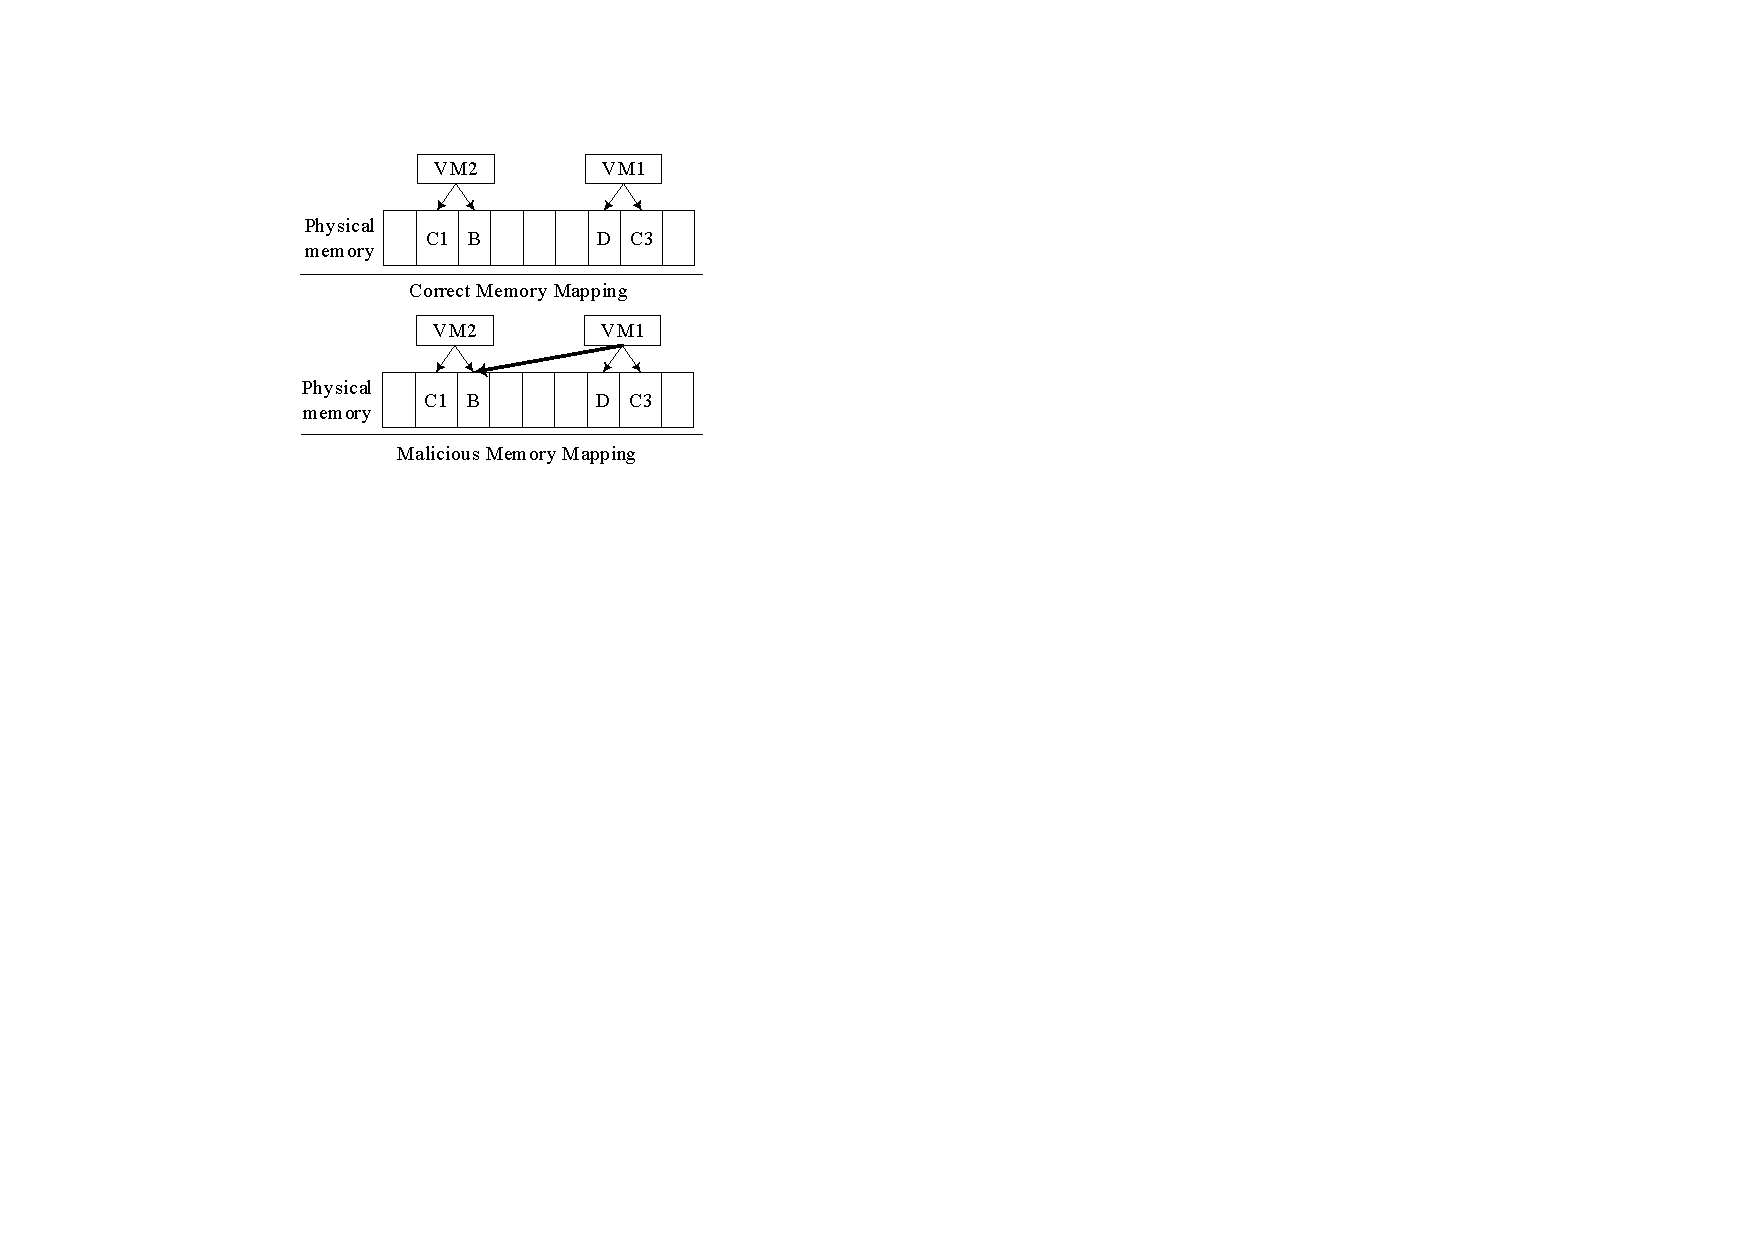
\includegraphics[width=0.8\linewidth]{IMG/remap.pdf}
    \caption{Diagram of Remapping Attack}
    \label{pic:remap}
\end{figure}

\textbf{Attacks to Kernel Page Tables}: 
We also take into account the fact that attacker already knows the deployment of HyperPS. As depicted in Figure \ref{fig:threat}, key components, such as Kernel Page Tables, Control Registers, to create the secure and isolated execution environment are also protected by us. We have designed mechanisms to validate the loaded values in HyperPS Space in case of potential attacks to them in the HostOS/Hypervisor Space.  
More details about the creation of the secure and isolated execution environment are illustrated in Section \ref{sub:hyperps_space}. 
%添加关于章节的引用
 


\subsection{Threat Model} \label{sub:threatmodel}
In this paper,  we do not care about how the adversary brings down the HostOS/Hypervisor. 
We assume that the Hostos/Hypervisor has been compromised and controlled by the powerful adversary.The adversary can turn off kernel security mechanisms, such as Date Execution Prevention(DEP), Supervisor Mode Execution Protection(SMEP), Supervisor Mode Access Prevention(SMAP), and so on.
We assume that the adversary does not possess the capability to conduct side channel attack and Hardware-based attack. We also assume that the adversary is unwilling to conduct the Denial of Service attack (DOS). In this paper, we assume that hardware resources are trusted, including processor, buses, BIOS/UEFI, and so on. 
We assume that if the adversary has acquired the memory locations where VMCS or EPTs locate at in the HostOS before. The adversary attempts to tamper fields in VMCSs and EPTs by using DMA write or regular memory access (access the memory with a pointer (e,g, memset or memcpy)). 
We do not limit the attack vector that how the adversary constructs payload to invoke DMA write and regular memory access functions. For example, the adversary can load a malicious loadable kernel module to overwrite VMCS fields with a pointer, the adversary can also construct a Code-Reuse-Attack (ROP, JOP, COOP, etc) payload to invoke functions that update Control Registers, VMCSes or EPTs. 
However, we do not consider instruction-level attacks. For example, we can not prevent the attacker from tampering VMCS or EPT with by executing the \verb|VMX| instruction directly. This is because that we can not hook instructions. Besides, some \verb|VMX| instructions, such as \verb|VMLAUNCH|, takes the VMCS identifier instead of a memory location as the input, which means the adversary does not need to know the current VMCS' memory location at all. 
% it does not rely on memory location. 
% field in these two data structures with \verb|VMX| instructions,  

% the adversary can tamper fields of VMCSs and EPTs through DMA write or regular memory access to them. 

% with dedicated malicious values. The adversary can also tamper VMCSs and EPTs through DMA write or regular memory access to them.  
% In details, if the adversary has acquired the memory locations where VMCS or EPTs locate at before,  

% we assume that the attacker can tamper these two data structures through direct memory write operations. The attacker can write these two data structures either through Direct Memory Access (DMA) or through regular memory access, if the attacker acquired these two data structures' memory locations before.  



% In details, we assume that the attacker can tamper VMCSs and EPTs with one of the following methods. First, the attacker can tamper any field in these two data structures with \verb|VMX| instructions, if the attacker has gained the root processor privilege. 
% Second, the attacker can tamper these two data structures through direct memory write operations. The attacker can write these two data structures either through Direct Memory Access (DMA) or through regular memory access, if the attacker acquired these two data structures' memory locations before.  
% We assume that 
% the adversary can tamper fields of VMCSs and EPTs with dedicated malicious values. The adversary can also tamper VMCSs and EPTs through DMA write or regular memory access to them.  

% We assume that the adversary does not possess the capability to conduct side channel attack and Hardware-based attack. We also assume that the adversary is unwilling to conduct the Denial of Service attack (DOS). In this paper, we assume that hardware resources are trusted, including processor, buses, BIOS/UEFI, and so on. 





















